% You should title the file with a .tex extension (hw1.tex, for example)
\documentclass[a4paper, 11pt]{article}

\usepackage{amsmath}
\usepackage{amssymb}
\usepackage{fancyhdr}
\usepackage{graphicx}

\usepackage[margin=1in]{geometry}

\newcommand{\question}[2] {\vspace{.25in} \hrule\vspace{0.5em}
\noindent{\bf #1: #2} \vspace{0.5em}
\hrule \vspace{.10in}}
\renewcommand{\part}[1] {\vspace{.10in} {\bf (#1)}}

\newcommand{\myname}{Natthakan Euaumpon}
\newcommand{\myemail}{natthakaneuaumpon@gmail.com}
\newcommand{\myhwnum}{3}

\setlength{\parindent}{0pt}
\setlength{\parskip}{5pt plus 1pt}
 
\pagestyle{fancyplain}
\lhead{\fancyplain{}{\textbf{HW\myhwnum}}}      % Note the different brackets!
\rhead{\fancyplain{}{\myname\\ \myemail}}
\chead{\fancyplain{}{ICCS310}}

\begin{document}

\medskip                        % Skip a "medium" amount of space
                                % (latex determines what medium is)
                                % Also try: \bigskip, \littleskip

\thispagestyle{plain}
\begin{center}                  % Center the following lines
{\Large ICCS310: Assignment \myhwnum} \\
\myname \\
\myemail \\
February 2021 \\
\end{center}

\question{1}{NFA vs DFA Expressiveness}
\part{1}\\
Let construct an NFA, $M = (Q,\Sigma,\delta,q_0,F) $ where $Q = \{0, 1, ..., k\}$. Let $\delta(0,b) = 0, \delta(0,1) = \{0,a\} = \{0,1\}$ and $\delta(i - 1, a) = i$, for $2 \leq i \leq k$. Then set $q_0 = 0$ and $F = \{k\}$. We know that the machine will start at state 0 (starting state). When the machine locate an $a$ it wil guess that it is a kth character to the right and will move to state 1. When it reaches state k, it will only accept if there are exactly $k-1$ bits following the one that move from $b$ to $a$.

\part{2}\\
Let the input have k character. We know that the characters can be either $a$ or $b$. Let $x$ and $y$ be a string with k bit such that $x,y \in \Sigma^*$ and that $|x| = |y| = k$. Let $i$ be a position such that $x_i \neq y_i$. Hence either $x$ or $y$ contain an a at the ith position. Let $z = b^{i-1}$, then $z$ distinguish $x$ and $y$ as one of the $xz$ and $yz$ has an a at kth postion from the right. Since there are $2^k$ string of length k that are all distinguishable from the above prove, a DFA that accept this language need to have $2^k$ states. 

\question{2}{Regular or Not}
\part{$L_1$}\\
We know that y can be any string in $\Sigma^*$. \\
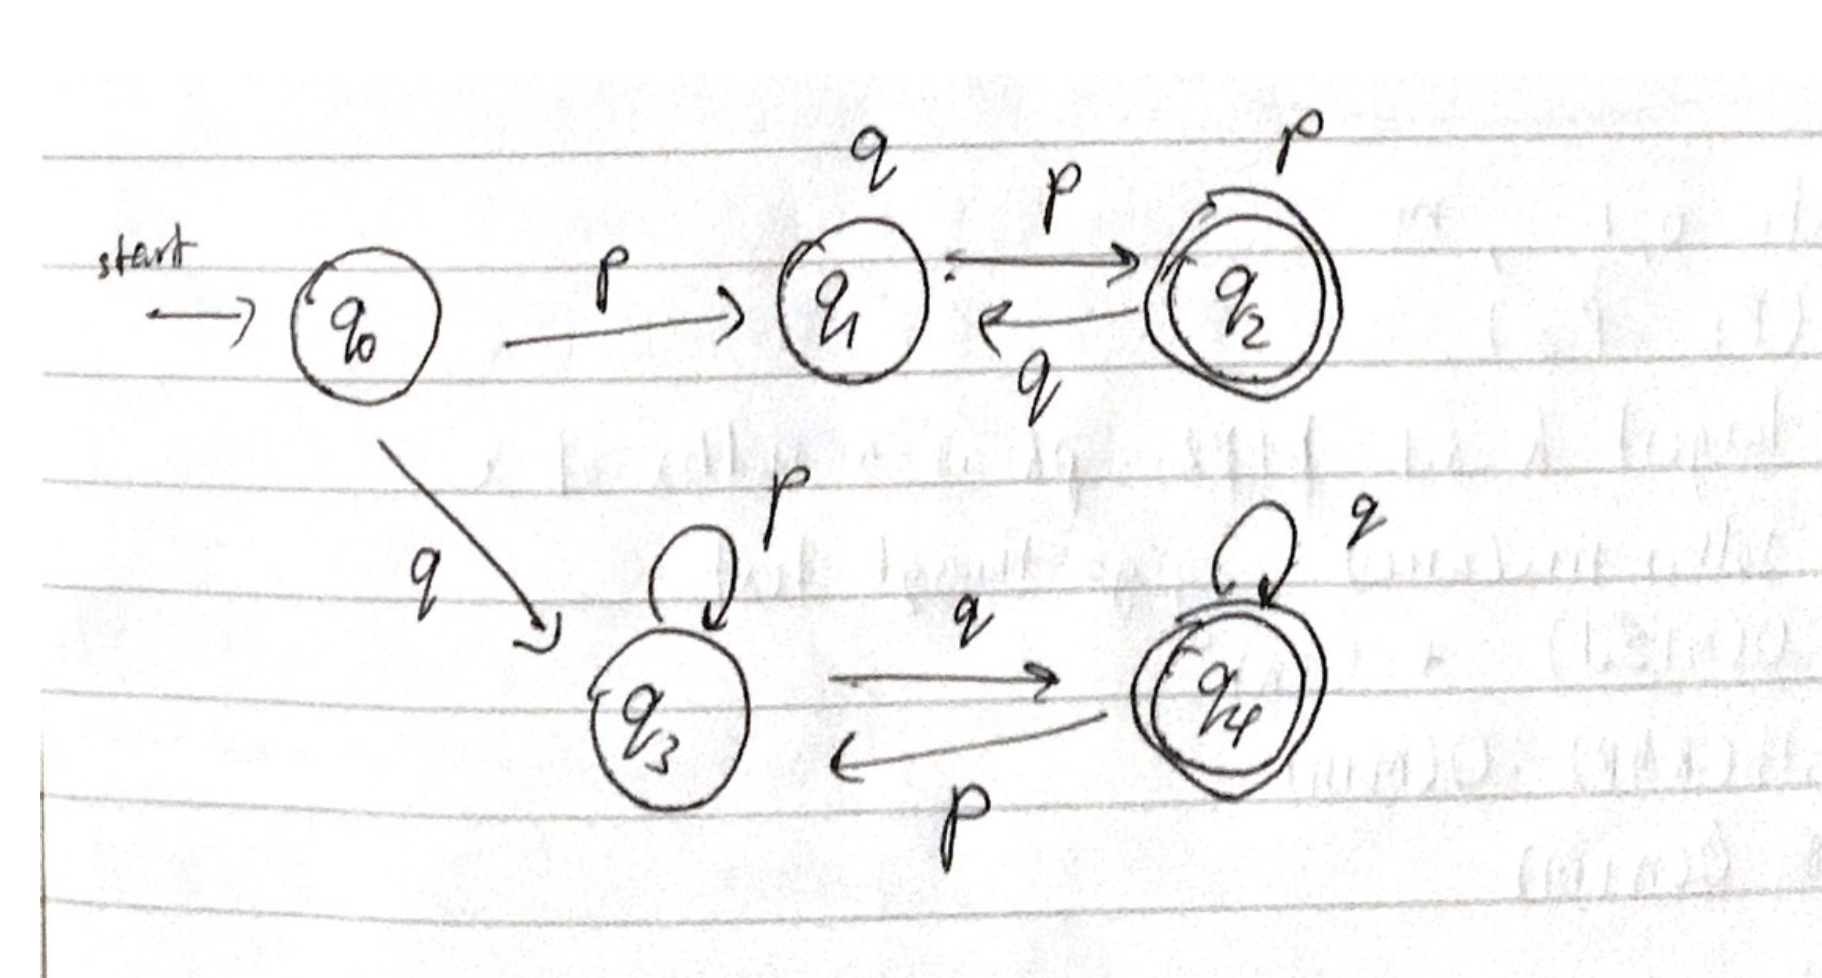
\includegraphics[width=\textwidth]{Q2-1-1.png}\\
There are 2 main scenario. One is that the String x start with p and another is that it start with q.\\
$q_0$ is a starting state.\\
$q_1$ is a state that it will move to if the first character is p.\\
$q_2$ is an accepting state, if the iput start with p then it should also end with p.\\
$q_3$ is a state that it will move to if the first character is q.\\
$q_4$ is an accepting state, if the iput start with q then it should also end with q.

\part{$L_2$}\\
AFSOC, that $L_2$ is regular. This mean their is a pumping length $l \geq 1$.  Consider string $S = p^lqqp^l$, $S \in L_2, |S| \geq l$. Since $S = ww^R$, where $w = p^lq$ then $S \in L_2$. From this we know that:
\begin{enumerate}
	\item S can be split into $S = xyz$
	\item $|xy| \leq l$
	\item $xy^iz \in L_2, i \geq 0$
	\item $xy = p^j$, $j \leq l$
	\item $y = p^k, k \geq 1$
\end{enumerate}
If we pump y 0 times then the string S will be $S = xz$. $xz = p^{l-k}qqp^l$. We state that $k \geq 1$, this mean $xz \notin L_2$. This contradict, therefore $L_2$ is not regular.

\question{3}{Nonregular}
\part{1}\\
AFSOC, that L is regular then their is a pumping length $p \geq 1$. Consider a string $S = 10^{2^p}, S \in L$. From this we know that:
\begin{enumerate}
	\item S can be split into $S = xyz$, and $xy$ be arbitary element in L.
	\item $|xy| \leq p$
	\item $xy^iz \in L, i \geq 0$
	\item $x = 10^{2^i}$
	\item $y = 10^{2^j}, 1 \leq j \leq i$
	\item Let $z = 10^{2^i}$
\end{enumerate}
From this we know that $xz = 10^{2^i} \cdot 10 ^{2^i}  = 10^{2^{i+1}}$, $xz \in L$. However $xy = 10^{2^i} \cdot 10^{2^j} = 10^{2^i+2^j}, xy \notin L$ as $i \neq j$. This contradict, therefore L is not regular.

\part{2}\\
AFSOC, that E is regular then their is a pumping length $p \geq 1$. Consider a string $S = $
\question{4}{HackerRank Challenge}
Natthakan Euaumpon\\
@natthakaneuaump1

\end{document}

